As we have discussed before, we would like to use uncertainty quantification to make predictions or infer information from real-life scenarios.
For example, a meteorologist would like to know the uncertainty in the weather predictions they make~\cite{kirkup2006}, a power grid operator might want to know more about the soil surrounding the cables~\cite{vanharten2025}, and an environmental specialist the flow of an underground aquifer~\cite{ballio2004}, to name a few.
All these examples require understanding some \emph{natural phenomenon}, which is frequently modeled using Partial Differential Equations (PDEs).

In this thesis, we will discuss uncertainty quantification for two partial differential equations: the \emph{Poisson equation} and the \emph{Helmholtz equation}, which we will introduce here.
We will start with the Laplace equation to derive the Poisson equation in Section~\ref{subsec:poisson-equation}.
Later, we will derive the Helmholtz equation from the linear wave equation in Section~\ref{subsec:helmholtz-equation}.

Finally, we will need a method to model the impact of uncertainty, which we will apply to partial differential equations.
Therefore, we will model uncertainty through a set of parameters on which the partial differential equations depend, and we will discuss this further in Section~\ref{subsec:paramterized-pdes}.

\subsection{Poisson equation}\label{subsec:poisson-equation}
The Laplace equation, first discovered by the French mathematician Pierre--Simon Laplace~\cite{laplace1798}, was introduced in the context of gravitational and electrostatic potentials, which satisfy the condition $\nabla^{2}u=0$.
In the twentieth century, the equation became central to the modeling of other natural phenomena, such as heat conduction, electrostatics, and elasticity.

Here, we will consider the Poisson equation, introduced by Siméon Denis Poisson around 1813.
This equation modifies the Laplace equation by considering a source term.
This source term models the distribution of sources and sinks for the potential.
It models, for example, the charge density in electrostatics, the mass in gravity, and the heat generation in steady-state heat conduction.
The Poisson equation is of elliptic type and is well-behaved in a mathematical sense.
This means that it has a unique solution that is continuously dependent on input data coming from the source term~\cite{evans2010}.

In this work, we will consider the \emph{heterogeneous Poisson equation} where the coefficients in the equation depend on the location in the bounded and connected domain $D\subset \mathbb{R}^d$ with $d\in\mathbb{N}$ (usually $d=1,2,3$ in applications).
We will consider \emph{Dirichlet boundary conditions} on the boundary to ensure a unique solution.
More precisely, the equation, together with the boundary condition, is given by:
\begin{equation*}
    \begin{cases}
        -\nabla  \cdot \left( A \nabla u \right) = f&\text{ in } D,\\
        u=0 & \text{ on }\partial D,
    \end{cases}
\end{equation*}
where $A \in \left(L^\infty(D)\right)^{d\times d}$ is the matrix-valued heterogeneous parameter and $f\in L^2(D)$ the source term discussed before.

\subsection{Helmholtz equation}\label{subsec:helmholtz-equation}
Next to the Poisson equation, we consider the Helmholtz equation.
However, before we discuss this, we will first introduce its parent, the wave equation, from which the Helmholtz equation will follow.
Then, having derived the Helmholtz equation, we introduce the Helmholtz scattering problem we will consider in this thesis.

\subsubsection{From the linear wave equation to the Helmholtz equation}
The wave equation is one of the earliest partial differential equations discovered.
Jean le Rond d'Alembert initially derived it for a one-dimensional vibrating string~\cite{dalembert1747}, which has been extended to two- and three-dimensional waves by Leonhard Euler to model membranes and fluids~\cite{euler1766}.
As the name suggests, the wave equation relates how a physical quantity varies in space and time as a wave propagates through a medium.
For example, this medium could be air, in the case of a loud neighbor, or the ground, in the case of an earthquake.
Hence, the wave equation combines time and spatial derivatives, forming a hyperbolic partial differential equation.
In its most simple form, it reads:
\begin{equation*}
    \frac{\partial^2 u(\x, t)}{\partial t^2} = c^2 \nabla^2 u(\x, t),\qquad \x\in D,
\end{equation*}
where $u(\x, t)$ is the quantity varying in space and time, $c$ the propagation speed and $D$ the domain.

Finding solutions to the wave equation can be rather challenging.
However, as is often the case, we can simplify the computations significantly using a well-placed ansatz.
In our case, we will assume that the solution $u$ is harmonic in time:
\begin{equation*}
    u(\x, t) \coloneqq \tilde{u}(\x)e^{-i\omega t},
\end{equation*}
where $\omega\in\mathbb{R}$ is the angular frequency and $i^2=-1$.
Substituting this ansatz into the wave equation and dividing out the time-dependent terms, we obtain
\begin{equation*}
    -\omega^2 \tilde{u}(\x) = c^2 \nabla^2 \tilde{u}(\x).
\end{equation*}
A little rearranging then arrives us at the \emph{Helmholtz equation}:
\begin{equation*}
    -\nabla^2 \tilde{u}(\x)-k^2\tilde{u}(\x) = 0,
\end{equation*}
where $k=\frac{c}{\omega}\in\mathbb{R}$ is the wave number.
Similarly to our treatment of the Poisson equation in Section~\ref{subsec:poisson-equation}, we will consider a generalization of the Helmholtz equation to take spatial inhomogeneities into account by introducing two heterogeneous coefficients $A$ and $n$:
\begin{equation*}
    -\nabla \cdot \left( A(\x) \nabla u(\x) \right)-k^2 n(\x)u(\x) = 0,
\end{equation*}
where we have dropped the redundant $\tilde{\cdot}$ above the $u$ to simplify notation.
The coefficient $n$ is generally known as the \emph{refractive index} of the medium and is assumed to be dependent on $\x$, and $A$ is a matrix-valued coefficient, also dependent on $\x$.

When we compare the Helmholtz equation with the Laplace equation presented in Section~\ref{subsec:poisson-equation}, we observe that the equations are very similar, except for the term $k^{2}u(\x)$.
This term makes the equation more difficult to solve, both analytically and numerically, and reflects the hyperbolic nature of the equation.
How much more difficult is greatly dependent on the wave number $k$, as the \emph{conditioning} of the problem becomes worse the higher $k$ becomes.

The Helmholtz equation is central to many other mathematical and physical domains.
Next to this time-harmonic ansatz of the wave equation, the Helmholtz equation follows from Maxwell's equations posed on linear, homogeneous, and isotropic media under a time-harmonic assumption~\cite[Chapter~2]{maier2007}.
Moreover, one can arrive at a similar equation through the Schrödinger equation~\cite[Chapter 10]{griffiths2018}.

\subsubsection{Exterior Helmholtz scattering}
In this thesis, we consider the Helmholtz equation for a two-dimensional scattering problem where an incoming wave $u_{in}$ interacts with a scatterer at the origin.
We thus pose the Helmholtz equation on the two-dimensional plane with a bounded impenetrable scatterer $D_{scat}$ centered at the origin with boundary $\Gamma_{scat}$.
At the boundary of the scatterer, the incoming wave exhibits \emph{sound-soft} scattering, modeling the central scatterer absorbing the incident wave.
The resulting configuration has been sketched schematically in Figure~\ref{fig:scat_tikz_R2}.

Furthermore, we assume that the coefficients $A$, $n$, and the domain define a \emph{non-trapping} problem.
This means, citing~\cite{graham2019}, that \emph{all billiard trajectories starting in an exterior neighborhood of the central scatterer and evolving according to the Hamiltonian flow defined by the coefficients $A$ and $n$ escape from that neighborhood after some uniform time.}
Intuitively, and as the name suggests, this implies that waves cannot get `trapped' in the cavities of the scatterer.
However, in the case of heterogeneous coefficients, this condition can become rather intricate, and we refer the reader to an overview in~\cite{graham2019}.

Finally, we impose the Sommerfeld radiation condition~\cite{sommerfeld1912}, enforcing that the outgoing wave decays the further we are from the scatterer at the origin, with rate $1/\sqrt {|\x|}$.
Combining everything, we arrive at the \emph{heterogeneous exterior scattering problem}:
\begin{equation*}
    \begin{cases}
        -\nabla \cdot \left( A \nabla u \right)-k^2 nu = 0, &\text{ in } D_{ext},\\
        u = 0, & \text{ on } \Gamma_{scat},\\
        \lim_{|\x|\to \infty} \sqrt {|\x|} \left( \frac{\partial}{\partial |\x|}  - ik\right) \left( u - u_{in} \right) = 0,
    \end{cases}
\end{equation*}
where the domain $D_{ext}=\mathbb{R}^2\setminus D_{scat}$.


\begin{figure}
    \centering
    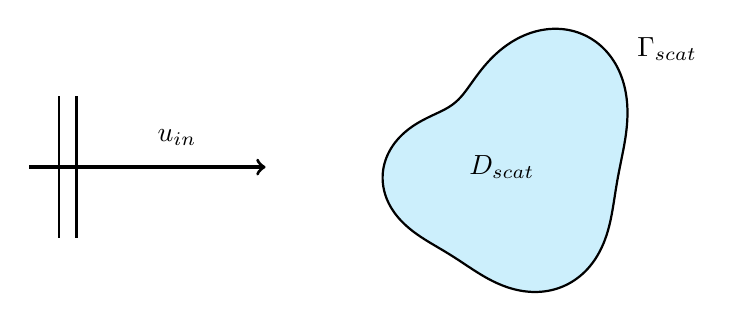
\begin{tikzpicture}[thick, scale=1.5]
        \draw[fill=cyan,domain=0:3*pi,samples=500,fill opacity=0.2] plot ({deg(\x)}:{((cos(\x * 1 r)^3 - cos(\x * 3 r) + sin(\x*2 r)*0.5)*0.2+1)});
        \draw[very thick, ->, >=to] (-4,0) -- (-2,0);
        \node[] at (-2.75, 0.25) {$u_{in}$};
        \draw[thick] (-3.75,-0.6) -- (-3.75,0.6);
        \draw[thick] (-3.6,-0.6) -- (-3.6,0.6);
        \node[] at (0,0) {$D_{scat}$};
        \node[] at (1.4,1) {$\Gamma_{scat}$};
    \end{tikzpicture}
    \caption{Schematic setting of the exterior Helmholtz scattering problem.}
    \label{fig:scat_tikz_R2}
\end{figure}


\subsection{Parameterized PDEs}\label{subsec:paramterized-pdes}
Thus far, we have just considered the \emph{deterministic} case, where the coefficients $A$ and $n$ and the source term $f$ are deterministic.
To consider the probabilistic aspect, we introduce a probability space $(\Omega, \mathcal{A}, \mathbb{P})$, where $\Omega$ is the set of events, $\mathcal{A}$ is a $\sigma$--algebra on the power set $\mathscr{P}(\Omega)$, and $\mathbb{P}$ the probability measure on $(\Omega,\mathcal{A})$.
For more details, see, for example,~\cite[Chapter~2]{sullivan2015}.
Hence, our target is to analyze \emph{random} partial differential equations where the coefficients and/or source term depend on some stochastic value $\omega$ taking values in $\Omega$.

We model this uncertainty through a parametric approach, where the coefficients and/or source term depend on a parameter $\y$ taking values in a parameter space $Y$.
The parameter space $Y$ is possibly infinite-dimensional, and in most of this work, we will consider hypercubes $Y=[-1,1]^{N}$, $N\in\mathbb{N}$ or $Y=[-1,1]^\mathbb{N}$.
hence, the probabilistic aspect can be treated by employing a suitable measure on $Y$, which describes the underlying randomness.
In the remainder of this work, we will restrict the discussion to the parameterized setting while recognizing that the probabilistic setting can be obtained by applying an appropriate measure on $Y$.

Taking this into account, we arrive at the following parameterized Poisson equation:
\begin{equation}
    \begin{cases}
        -\nabla  \cdot \left( A(\y) \nabla u(\y) \right) = f(\y),&\text{ in } D,\\
        u(\y)=0, & \text{ on }\partial D,\\
        \text{for every }\y\in Y,
    \end{cases}\label{eq:parameterized_poisson_pde}
\end{equation}
where the gradient is taken with respect to the omitted spatial variable and where, for every $\y \in Y$, $A(\y) \in \left(L^\infty(D)\right)^{d\times d}$ and $f\in L^2(D)$ with parameter-independent bounds in their respective norms.
Moreover, we require that $A(\y, \cdot)$ is positive definite with respect to both the spatial coordinate and the parameter.

In a similar fashion, we obtain the following parameterized exterior Helmholtz scattering problem:
\begin{equation}
    \begin{cases}
        -\nabla \cdot \left( A(\y) \nabla u(\y) \right)-k^2 n(\y)u(\y) = 0, &\text{ in } D_{ext},\\
        u(\y) = 0, & \text{ on } \Gamma_{scat},\\
        \lim_{|\x|\to \infty} \sqrt {|\x|} \left( \frac{\partial}{\partial |\x|}  - ik\right) \left( u(\y) - u_{in} \right) = 0,\\
        \text{for every }\y\in Y,
    \end{cases}\label{eq:parameterized_helmholtz_pde}
\end{equation}
where, again, for every $\y \in Y$, $A(\y) \in \left(L^\infty(D)\right)^{2\times 2}$ is positive definite, uniformly with respect to both variables and $n(\y)$ is the heterogeneous, positive, real-valued refractive index of the medium.

Later in this work, we will consider PDEs posed on a parametric domain.
As we will show, this case will reduce to the parametric equations~\eqref{eq:parameterized_poisson_pde} and~\eqref{eq:parameterized_helmholtz_pde}.
Parametric PDEs can also be found beyond the scope of UQ, for example, in optimization and control applications.

\subsection{Numerical approximations}\label{subsec:finite-element-approximations}
Solving partial differential equations analytically is a notoriously involved task.
We can employ techniques such as separation of variables, transformation methods like Fourier or Laplace transforms, or Green's functions on simple domains, such as rectangles or circles, with piecewise constant coefficients~\cite[Chapters~2 and~4]{evans2010}.

For PDEs with heterogeneous coefficients or domains with more complex geometries, analytic techniques quickly become infeasible.
Therefore, we will employ, for given $\y\in Y$, the \emph{Finite element method}~\cite{brenner2008}, in which we project our equation into a finite-dimensional subspace in which we search for the PDE solution.
This finite-dimensional approximation then allows us to formulate the problem as a \emph{linear system}, which we can treat using techniques from linear algebra.
We will briefly outline this process in the upcoming paragraphs.

\subsubsection{Poisson equation}
First, we will treat the Poisson equation~\eqref{eq:parameterized_poisson_pde}.
Before we can project onto the finite-dimensional approximation space, we must derive the \emph{variational form} of equation~\eqref{eq:parameterized_poisson_pde}.
We do this by multiplying with a suitably smooth \emph{test function} $v\in V\coloneqq H_0^1(D)$, and integrating over the spatial domain to obtain the variational formulation:

Find, for all $\y\in Y$, $u\in V$ such that
\begin{equation}
    \int_D A(\y) \nabla u(\y) \cdot \nabla v \dx = \int_D f(\y)v \dx\label{eq:varformpoisson},
\end{equation}
for all $v\in V$ where $V=H_0^1(D)$.

\begin{figure}
    \centering
    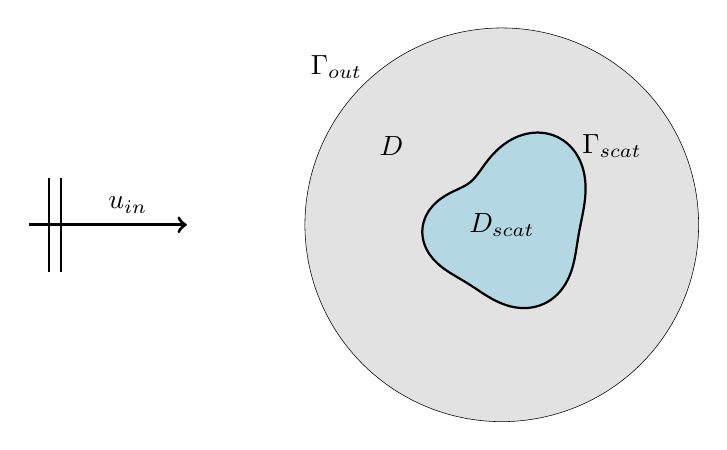
\begin{tikzpicture}[thick]
        \draw[fill=lightgray!45,domain=0:2*pi,samples=500,very thin] plot ({deg(\x)}:{2.5});
        \draw[fill=cyan,domain=0:3*pi,samples=500,fill opacity=0.2] plot ({deg(\x)}:{((cos(\x * 1 r)^3 - cos(\x * 3 r) + sin(\x*2 r)*0.5)*0.2+1)});
        \draw[very thick, ->, >=to] (-6,0) -- (-4,0);
        \node[] at (-4.75, 0.25) {$u_{in}$};
        \draw[thick] (-5.75,-0.6) -- (-5.75,0.6);
        \draw[thick] (-5.6,-0.6) -- (-5.6,0.6);
        \node[] at (0,0) {$D_{scat}$};
        \node[] at (1.4,1) {$\Gamma_{scat}$};
        \node[] at (-2.1,2) {$\Gamma_{out}$};
        \node[] at (-1.4,1) {$D$};
    \end{tikzpicture}
    \caption{Schematic setting of the truncated Helmholtz scattering problem.}
    \label{fig:scat_tikz}
\end{figure}


\subsubsection{Exterior Helmholtz scattering}
We want to derive a variational formulation for the Helmholtz scattering case by employing a similar technique.
However, we first need to address the fact that $D_{ext}$ is unbounded before we can impose the Sommerfeld radiation condition.
To achieve this, we introduce a circle $\Gamma_{out}$ with radius $r_{out}$ containing the scatterer $D_{scat}$.
With this circle at hand, we truncate the unbounded domain $D_{ext}$ to get the computational domain
\begin{equation*}
    D = \left\{ \x \in D_{scat} :\, |\x| < r_{out} \right\}.
\end{equation*}
Figure~\ref{fig:scat_tikz} depicts the resulting configuration.
At the outer boundary $\Gamma_{out}$, we have to approximate the Sommerfeld radiation condition, for which we can take one of several approaches.

First, we could compute the exact \emph{Dirichlet-to-Neumann} (DtN) map at the boundary and use it to implement the boundary condition~\cite[Section~2.5]{nedelec2001}.
Using the DtN map is exact and would be the preferred option.
However, finding an analytic expression for the DtN map is notoriously challenging and can only be done in basic cases for relatively simple equations.
Therefore, this approach is not feasible for our current needs.

On the other hand, we could implement a \emph{Perfectly matched layer} (PML) around our computational domain that absorbs the scattered wave with little reflection~\cite{collino1998,berenger2007}.
This absorption is performed using complex coordinate stretching, which is dependent on, among other things, the damping profile and the layer thickness.
The thickness of the layer and the damping profile must be carefully chosen to ensure the PML performs optimally, which may require some fine-tuning.
Moreover, the PML enlarges the computational domain, increasing the overall computational cost.

A more straightforward method is to impose the far-field Sommerfeld condition at the computational boundary $\Gamma_{out}$.
This approach works well when the scattered waves move outwards in the normal direction to $\Gamma_{out}$, and the outer edge of the computational domain is simple.
It is less accurate than the previously mentioned methods, but it does not impact computational performance and is straightforward to implement.
Hence, we employ this method by imposing a Robin boundary condition on $\Gamma_{out}$:
\begin{equation}
    \begin{cases}
        -\nabla \cdot \left( A(\y) \nabla u(\y) \right)-k^2 n(\y)u(\y) = 0, &\text{ in } D,\\
        u(\y) = 0, & \text{ on } \Gamma_{scat},\\
        \left( \frac{\partial}{\partial\bm{n}} -ik\right)\left( u(\y)-u_{in} \right) = 0, & \text{ on } \Gamma_{out},\\
        \text{for every }\y\in Y,
    \end{cases}\label{eq:parameterized_helmholtz_pde_truncated}
\end{equation}
where $\bm{n}$ is the unit normal vector to $\Gamma_{out}$, pointing outwards.
Having made this truncation, we can finally formulate the variational form:

Find, for all $\y\in Y$, $u(\y) \in V$:
\begin{align}
    \int_D A(\y) \nabla u(\y) \cdot \nabla v \dx &-k^2\int_D n(\y)  u(\y) v \dx -ik\int_{\Gamma_{out}} u(\y) v \dx \nonumber\\
    &= \int_{\Gamma_{out}} \left( \frac{\partial}{\partial\bm{n}} -ik\right) u_{in} v \dx.\label{eq:varformhelmholtz}
\end{align}
for all $v\in V$ with $V=H^1_{0, \Gamma_{scat}}(D)$.

\subsubsection{Finite element method}
With these variational formulations at hand, we approximate both the solution space $V$ and the test space $V$ with a finite-dimensional approximation $V_h\subset V$ with basis $\left\{ \phi_j(\x) \right\}$ consisting of $N_{\mathrm{dof}}$ degrees of freedom.
Standard choices of bases for $V_h$ are, for example, linear basis functions (colloquially known as the hat functions), piecewise constant functions, or higher-order polynomial basis functions.
However, crucially, there are a finite number of basis functions, which gives the method its name.

For the Poisson equation, we now approximate $u(\y)$ by the finite element approximation $u_h(\y)=\sum_{i}u_i(\y)\phi_i\in V_h$, and insert it into the variational form~\eqref{eq:varformpoisson} to obtain
\begin{equation*}
    \sum_{i} u_i(\y) \int_D A(\y) \nabla \phi_i  \cdot \nabla v \dx = \int_D f(\y)v \dx.
\end{equation*}
Now, we test this equation with $v=\phi_j$ for each test function to obtain a linear system of equations
\begin{equation*}
    \mathbb{A}(\y)\bm{u}(\y)=F(\y),
\end{equation*}
where $\u(\y)\in\mathbb{R}^{N_{\mathrm{dof}}}$ such that $\bm{u}(\y)_i = u_i(\y)$,
\begin{equation*}
[\mathbb{A}(\y)]_{ij}=\int_D A(\y) \nabla \phi_i  \cdot \nabla \phi_j \dx, \qquad i,j=1,\ldots, N_{\mathrm{dof}},
\end{equation*}
and
\begin{equation*}
    F_i(\y) = \int_D f(\y) \phi_j \dx, \qquad i=1,\ldots, N_{\mathrm{dof}}.
\end{equation*}
We can treat the variational formulation of the Helmholtz equation in~\eqref{eq:varformhelmholtz} similarly with $V_h\subset V=H^1_{0, \Gamma_{scat}}(D)$, leading to a system of linear equations with the same form but with different entries.

To summarize, we introduced two parameterized partial differential equations, the Poisson and Helmholtz equations.
Furthermore, we have discussed a computational method to approximate their solutions using the finite element method for any value of the parameter $\y$.

With these forward models, we can progress towards the next step, quantifying the effects of uncertainty on the solutions of these partial differential equations.